%iffalse
\let\negmedspace\undefined
\let\negthickspace\undefined
\documentclass[journal,12pt,onecolumn]{IEEEtran}
\usepackage{cite}
\usepackage{amsmath,amssymb,amsfonts,amsthm}
\usepackage{algorithmic}
\usepackage{graphicx}
\usepackage{textcomp}
\usepackage{xcolor}
\usepackage{txfonts}
\usepackage{listings}
\usepackage{enumitem}
\usepackage{enumitem,multicol}
\usepackage{mathtools}
\usepackage{gensymb}
\usepackage{comment}
\usepackage[breaklinks=true]{hyperref}
\usepackage{tkz-euclide} 
\usepackage{listings}
\usepackage{gvv}                                        
%\def\inputGnumericTable{}                                 
\usepackage[latin1]{inputenc}                                
\usepackage{color}                                            
\usepackage{array}                                            
\usepackage{longtable}                                       
\usepackage{calc}                                             
\usepackage{multirow}                                         
\usepackage{hhline}                                           
\usepackage{ifthen}                                           
\usepackage{lscape}
\usepackage{tabularx}
\usepackage{array}
\usepackage{float}
\usepackage[american,siunitx]{circuitikz}
\usetikzlibrary{arrows,shapes,calc,positioning}
\usepackage{pgfplots}


\newtheorem{theorem}{Theorem}[section]
\newtheorem{problem}{Problem}
\newtheorem{proposition}{Proposition}[section]
\newtheorem{lemma}{Lemma}[section]
\newtheorem{corollary}[theorem]{Corollary}
\newtheorem{example}{Example}[section]
\newtheorem{definition}[problem]{Definition}
\newcommand{\BEQA}{\begin{eqnarray}}
\newcommand{\EEQA}{\end{eqnarray}}
\newcommand{\define}{\stackrel{\triangle}{=}}
\theoremstyle{remark}
\newtheorem{rem}{Remark}
\pgfplotsset{compat=1.18}

% Marks the beginning of the document
\begin{document}
\bibliographystyle{IEEEtran}
\vspace{3cm}

\title{AE-2022}
\author{EE24Btech11022 - Eshan Sharma}
\maketitle

\renewcommand{\thefigure}{\theenumi}
\renewcommand{\thetable}{\theenumi}



\begin{enumerate}
\item The point of maximum entropy on a Fanno-curve in a Temperature-Entropy (T-s) diagram represents the
\begin{enumerate}
	\item maximum flow Mach number
	\item minimum flow Mach number
	\item sonic Mach number
	\item normal shock in the flow
\end{enumerate}

\item Consider a two-dimensional potential flow over a cylinder. If the freestream speed is $U_{\infty}$, the maximum speed on the cylinder surface is
\begin{enumerate}
	\item $\frac{U_{\infty}}{2}$
	\item $\frac{3 U_{\infty}}{2}$
	\item $2 U_{\infty}$
	\item $\frac{4 U_{\infty}}{3}$
\end{enumerate}

\item Consider steady, two-dimensional, incompressible flow over a non-porous flat plate as shown in the figure. For the control volume PQRS, the speed, $U_{\infty}$, at section PQ is uniform and the speed at section RS is given by 
\[
u(y) = A_0 \brak{\frac{y}{h}}^n,
\]
where $n$ is a positive integer. The value of $A_0$ for which the flow through section PS will $vanish$ is:

\begin{figure}[!ht]
	\centering
	\resizebox{0.8\textwidth}{!}{
		\begin{circuitikz}
			\tikzstyle{every node}=[font=\Large]
			\draw [line width=0.8pt, short] (7.5,11.25) -- (7.5,16.75);
			\draw [line width=0.8pt, short] (19.25,11.25) -- (19.25,16.75);
			\draw [line width=2pt, short] (7.5,11.25) -- (19.25,11.25);
			\draw [line width=1pt, ->, >=Stealth] (7.5,16.75) -- (23,16.75);
			\draw [line width=0.8pt, short] (19.25,11.25) .. controls (22.25,12) and (22.5,14) .. (23,16.75);
			\draw [line width=1pt, ->, >=Stealth] (19.25,15.5) -- (22.75,15.5);
			\draw [line width=1pt, ->, >=Stealth] (19.25,14.25) -- (22.25,14.25);
			\draw [line width=1pt, ->, >=Stealth] (19.25,13) -- (21.75,13);
			\draw [line width=1pt, ->, >=Stealth] (19.25,12) -- (20.75,12);
			\draw [line width=1pt, ->, >=Stealth] (7.5,16.75) -- (8.5,16.75);
			\draw [line width=1pt, ->, >=Stealth] (7.5,15.5) -- (8.5,15.5);
			\draw [line width=1pt, ->, >=Stealth] (7.5,14.25) -- (8.5,14.25);
			\draw [line width=1pt, ->, >=Stealth] (7.5,13) -- (8.5,13);
			\draw [line width=1pt, ->, >=Stealth] (7.5,12) -- (8.5,12);
			\draw [line width=1pt, ->, >=Stealth] (5.25,11.25) -- (5.25,12.75);
			\draw [line width=1pt, ->, >=Stealth] (5.25,11.25) -- (6.5,11.25);
			\draw [line width=1pt, <->, >=Stealth] (15.5,16.75) -- (15.5,11.25);
			\node [font=\Large] at (7.5,17.5) {P};
			\node [font=\Large] at (7.5,10.25) {Q};
			\node [font=\Large] at (19.25,10.5) {R};
			\node [font=\Large] at (19.25,17.5) {S};
			\node [font=\LARGE] at (6,13.5) {$u_\infty$};
			\node [font=\Large] at (4.75,12) {y};
			\node [font=\Large] at (6.25,10.75) {x};
			\node [font=\Large] at (14.75,13.75) {h};
			\node [font=\LARGE] at (24.25,13.25) {$u(y) = A_0 \brak{\frac{y}{h} }^n$};
		\end{circuitikz}
	}
\end{figure}

\begin{enumerate}
	\item $\frac{U_{\infty}}{n+1}$
	\item $U_{\infty}(n+1)$
	\item $\frac{U_{\infty}}{n-1}$
	\item $U_{\infty}(n-1)$
\end{enumerate}

\item Consider the velocity distribution, $u\brak{y}$ shown in the figure. For two adjacent fluid layers $L1$ and $L2$, the viscous force exerted by $L1$ on $L2$ is

\begin{center}
		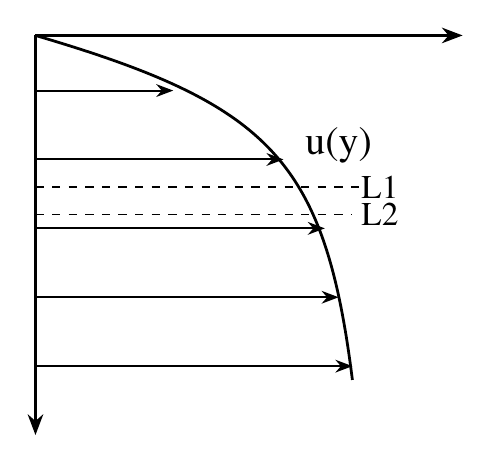
\begin{tikzpicture}[scale = 0.7]
			\tikzstyle{every node}=[font=\Large]
			\draw [line width=1pt, ->, >=Stealth] (11.5,16.5) -- (11.5,9.25);
			\draw [line width=1pt, ->, >=Stealth] (11.5,16.5) -- (19.25,16.5);
			\draw [line width=1pt, short] (11.5,16.5) .. controls (15.75,15.25) and (16.75,14.25) .. (17.25,10.25);
			\draw [line width=0.7pt, ->, >=Stealth] (11.5,15.5) -- (14,15.5);
			\draw [line width=0.7pt, ->, >=Stealth] (11.5,14.25) -- (16,14.25);
			\draw [line width=0.7pt, ->, >=Stealth] (11.5,13) -- (16.75,13);
			\draw [line width=0.7pt, ->, >=Stealth] (11.5,11.75) -- (17,11.75);
			\draw [line width=0.7pt, ->, >=Stealth] (11.5,10.5) -- (17.25,10.5);
			\draw [line width=0.6pt, dashed] (11.5,13.75) -- (17.5,13.75);
			\draw [line width=0.6pt, dashed] (11.5,13.25) -- (17.25,13.25);
			\node [font=\Large] at (17,14.5) {u(y)};
			\node [font=\large] at (17.75,13.75) {L1};
			\node [font=\large] at (17.75,13.25) {L2};
		\end{tikzpicture}
\end{center}

\begin{enumerate}
	\item to the right
	\item to the left
	\item vertically upwards
	\item vertically downwards
\end{enumerate}

\item The service ceiling of an airplane is the altitude
\begin{enumerate}
	\item at which maximum rate of climb is 100 m/min
	\item beyond which theoretically the airplane cannot sustain level flight
	\item at which maximum power is required for flight
	\item at which maximum rate of climb is 100 ft/min
\end{enumerate}
	
\item Regarding the horizontal tail of a conventional airplane, which one of the following statements is true?
\begin{enumerate}
	\item It contributes to $C_{m_{\alpha}} < 0$
	\item It makes $C_{m_{\alpha}} = 0$
	\item It makes $C_{m_{\alpha}} > 0$
	\item It makes $C_{m_0} > 0$ and $C_{m_{\alpha}} > 0$
\end{enumerate}

\item A beam with symmetrical T-shaped cross-section, as shown in the figure, is subjected to pure bending. The maximum magnitude of the normal stress is realised:

\begin{figure}[!ht]
	\centering
	\resizebox{0.8\textwidth}{!}{
		\begin{circuitikz}
			\tikzstyle{every node}=[font=\Large]
			\draw [ line width=0.6pt ] (10,14) -- (23.25,14) -- (22.75,13.5) -- (9.5,13.5) -- cycle;
			\draw [ line width=0.6pt ] (9.5,13.5) rectangle (22.75,13.25);
			\draw [ line width=0.6pt ] (9.5,13.25) rectangle (22.75,12.25);
			\draw [->, >=Stealth] (9,12.25) .. controls (8,12.75) and (8.25,13.25) .. (9,13.75) ;
			\draw [->, >=Stealth] (24,12.25) .. controls (24.75,12.75) and (24.75,13.25) .. (24,13.75) ;
			\node [font=\LARGE] at (7.5,13) {M};
			\node [font=\LARGE] at (23.5,12.75) {M};
			\node [font=\LARGE] at (16.25,14.5) {Top};
			\node [font=\LARGE] at (15.75,11.25) {Bottom};
			\draw  (25.5,15.25) rectangle (30.5,11);
			\draw  (26.75,13.25) rectangle (29,13);
			\draw  (27.75,13) rectangle (28,11.75);
			\node [font=\Large] at (27.75,14.5) {Cross-section};
		\end{circuitikz}
	}
\end{figure}

\begin{enumerate}
	\item only at the top fibres of the cross-section
	\item only at the bottom fibres of the cross-section
	\item both at the top and bottom fibres of the cross-section
	\item only at the centroidal fibres of the cross-section
\end{enumerate}

\item A three-member truss is simply supported at $\vec{Q}$ and $\vec{R}$, and loaded at $\vec{P}$ by a horizontal force $F$ as shown. The force in $QR$ is

\begin{center}
	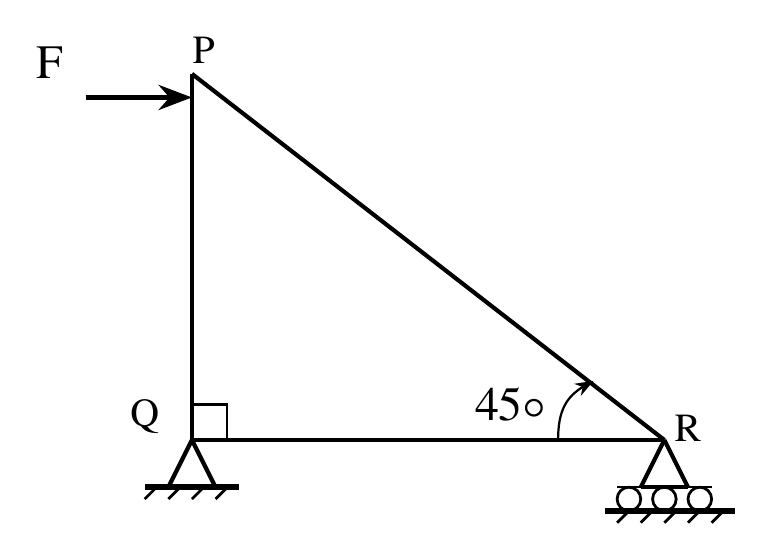
\begin{tikzpicture}[scale = 0.6]
			\tikzstyle{every node}=[font=\LARGE]
			\draw [line width=1.5pt, short] (15.5,16.5) -- (15.5,8.75);
			\draw [line width=1.5pt, short] (15.5,8.75) -- (25.5,8.75);
			\draw [line width=1.5pt, short] (15.5,16.5) -- (25.5,8.75);
			\draw [line width=1.5pt, short] (15.5,8.75) -- (15,7.75);
			\draw [line width=1.5pt, short] (15.5,8.75) -- (16,7.75);
			\draw [line width=1.5pt, short] (15,7.75) -- (16,7.75);
			\draw [line width=1.5pt, short] (25.5,8.75) -- (25,7.75);
			\draw [line width=1.5pt, short] (25.5,8.75) -- (26,7.75);
			\draw [line width=1.5pt, short] (25,7.75) -- (26,7.75);
			\draw [line width=2pt, short] (14.5,7.75) -- (16.5,7.75);
			\draw [ line width=1pt ] (24.75,7.5) circle (0.25cm);
			\draw [ line width=1pt ] (25.5,7.5) circle (0.25cm);
			\draw [ line width=1pt ] (26.25,7.5) circle (0.25cm);
			\draw [line width=2pt, short] (24.25,7.25) -- (27,7.25);
			\draw [line width=2pt, ->, >=Stealth] (13.25,16) -- (15.5,16);
			\draw [line width=1pt, short] (14.75,7.75) -- (14.5,7.5);
			\draw [line width=1pt, short] (15.25,7.75) -- (15,7.5);
			\draw [line width=1pt, short] (15.75,7.75) -- (15.5,7.5);
			\draw [line width=1pt, short] (16.25,7.75) -- (16,7.5);
			\draw [line width=1pt, short] (24.75,7.25) -- (24.5,7);
			\draw [line width=1pt, short] (25.25,7.25) -- (25,7);
			\draw [line width=1pt, short] (25.75,7.25) -- (25.5,7);
			\draw [line width=1pt, short] (26.25,7.25) -- (26,7);
			\draw [line width=1pt, short] (26.75,7.25) -- (26.5,7);
			\draw [ line width=0.8pt ] (15.5,9.5) rectangle (16.25,8.75);
			\draw [line width=0.8pt, ->, >=Stealth] (23.25,8.75) .. controls (23.25,9.5) and (23.5,9.75) .. (24,10) ;
			\draw [line width=0.8pt, short] (24.5,7.75) -- (26.5,7.75);
			\node [font=\Large] at (14.5,9.25) {Q};
			\node [font=\Large] at (26,9) {R};
			\node [font=\Large] at (15.75,17) {P};
			\node [font=\LARGE] at (12.5,16.75) {F};
			\node [font=\LARGE] at (22.25,9.5) {45$\circ$};
	\end{tikzpicture}
\end{center}

\begin{enumerate}
	\item 0
	\item $F\brak{tensile}$
	\item $\frac{F}{\sqrt{2}}\brak{compressive}$
	\item $\sqrt{2}F\brak{tensile}$
\end{enumerate}

\item The closed $thin-walled$ rectangular channel shown in figure $\brak{i}$ is opened by introducing a sharp cut at the center of the bottom edge, as shown in the figure $\brak{ii}$. Which of the following statements is correct?

\begin{figure}[!ht]
	\centering
	\resizebox{0.6\textwidth}{!}{
		\begin{circuitikz}
			\tikzstyle{every node}=[font=\LARGE]
			\draw [ line width=2pt ] (10.5,14.5) rectangle (19,9.75);
			\draw [line width=2pt, short] (22.5,14.5) -- (31,14.5);
			\draw [line width=2pt, short] (22.5,14.5) -- (22.5,9.75);
			\draw [line width=2pt, short] (22.5,9.75) -- (26.5,9.75);
			\draw [line width=2pt, short] (31,14.5) -- (31,9.75);
			\draw [line width=2pt, short] (27,9.75) -- (31,9.75);
			\draw [line width=0.9pt, ->, >=Stealth] (26.25,11.5) -- (26.75,10);
			\node [font=\LARGE] at (25.75,12) {cut};
			\node [font=\LARGE] at (15,15) {2a};
			\node [font=\LARGE] at (10,12.25) {b};
			\node [font=\LARGE] at (19.5,12) {b};
			\node [font=\LARGE] at (14.75,9.25) {2a};
			\node [font=\LARGE] at (26.75,15) {2a};
			\node [font=\LARGE] at (21.5,12.25) {b};
			\node [font=\LARGE] at (31.5,12) {b};
			\node [font=\LARGE] at (24.25,9.25) {a};
			\node [font=\LARGE] at (29.25,9.25) {a};
			\node [font=\LARGE] at (9.25,14.75) {(i)};
			\node [font=\LARGE] at (21.75,14.75) {(ii)};
		\end{circuitikz}
	}
\end{figure}

\begin{enumerate}
	\item centroids of $\brak{i}$ and $\brak{ii}$ coincide while shear centers do not
	\item shear centers of $\brak{i}$ and $\brak{ii}$ coincide while centroids do not
	\item Both centroids and shear centers of $\brak{i}$ and $\brak{ii}$ coincide
	\item Neither centroids nor shear centers of $\brak{i}$ and $\brak{ii}$ coincide
\end{enumerate}

\item The region of \textit{highest static temperature} in a rocket engine and the region of \textit{highest heat flux} are \_\_\_\_\_\_\_\_\_, respectively.

\begin{enumerate}
	\item nozzle throat and nozzle entry 
	\item combustion chamber and nozzle throat
	\item nozzle exit and nozzle throat
	\item nozzle throat and combustion chamber
\end{enumerate}

\item If $\hat{a}$, $\hat{b}$, $\hat{c}$ are three mutually perpendicular unit vectors, then $\hat{a} \cdot (\hat{b} \times \hat{c})$ can take the value(s):

\begin{enumerate}
	\item $0$
	\item $1$
	\item $-1$
	\item $\infty$
\end{enumerate}

\item Across an oblique shock wave in a calorifically perfect gas,

\begin{enumerate}
	\item the stagnation enthalpy changes
	\item the stagnation entropy changes
	\item the stagnation temperature changes
	\item the speed of sound changes
\end{enumerate}

\item NACA 2412 airfoil has

\begin{enumerate}
	\item 4\% maximum camber with respect to chord
	\item maximum camber at 40\% chord
	\item 12\% maximum thickness to chord ratio
	\item maximum camber at 20\% chord
\end{enumerate}



\end{enumerate}
\end{document}


